\documentclass[tikz,border=2pt]{standalone}
\usepackage{amsmath,amssymb}
\usepackage{tikz}
\usetikzlibrary{arrows.meta}

\begin{document}
% On a connected set E a continuous real-valued f cannot skip values: every y between f(a)
% and f(b) is attained at some point c of E (here on a path from a to b).
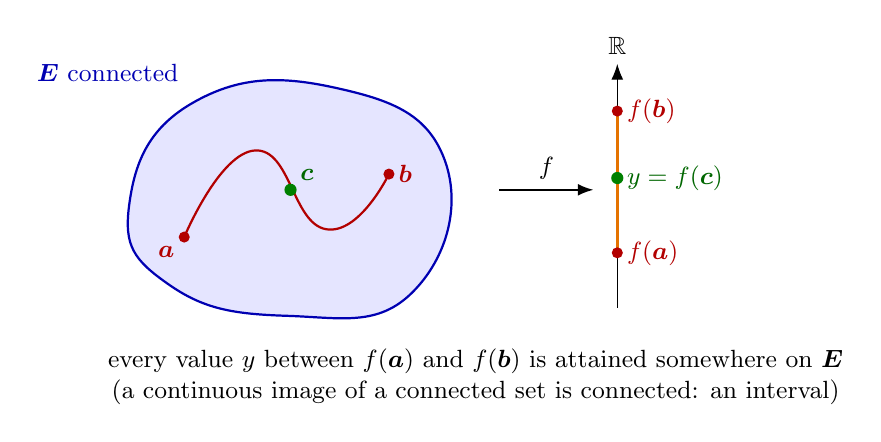
\begin{tikzpicture}[every node/.style={font=\small}, >={Latex[length=2mm]}]
	\fill[blue!10] plot[smooth cycle, tension=0.8] coordinates {(-2,0) (-1.2,1.3) (0.6,1.5) (2,0.6) (1.6,-1.1) (0,-1.4) (-1.5,-1)};
	\draw[blue!70!black, thick] plot[smooth cycle, tension=0.8] coordinates {(-2,0) (-1.2,1.3) (0.6,1.5) (2,0.6) (1.6,-1.1) (0,-1.4) (-1.5,-1)};
	\node[blue!70!black, anchor=south east] at (-1.25,1.45) {$\boldsymbol{E}$ connected};
	\draw[red!70!black, thick] plot[smooth, tension=0.9] coordinates {(-1.3,-0.4) (-0.4,0.7) (0.5,-0.3) (1.3,0.4)};
	\fill[red!70!black] (-1.3,-0.4) circle (2pt) node[below left] {$\boldsymbol{a}$};
	\fill[red!70!black] (1.3,0.4) circle (2pt) node[right] {$\boldsymbol{b}$};
	\fill[green!50!black] (0.05,0.2) circle (2.2pt) node[above right, green!40!black] {$\boldsymbol{c}$};
	\draw[->, thick] (2.7,0.2) -- (3.9,0.2) node[midway, above] {$f$};
	\begin{scope}[xshift=4.4cm]
		\draw[->] (-0.2,-1.3) -- (-0.2,1.8) node[above] {$\mathbb{R}$};
		\draw[very thick, orange!90!black] (-0.2,-0.6) -- (-0.2,1.2);
		\fill[red!70!black] (-0.2,-0.6) circle (2pt) node[right] {$f(\boldsymbol{a})$};
		\fill[red!70!black] (-0.2,1.2) circle (2pt) node[right] {$f(\boldsymbol{b})$};
		\fill[green!50!black] (-0.2,0.35) circle (2.2pt) node[right, green!40!black] {$y=f(\boldsymbol{c})$};
	\end{scope}
	\node[anchor=north, align=center] at (2.4,-1.7) {every value $y$ between $f(\boldsymbol{a})$ and $f(\boldsymbol{b})$ is attained somewhere on $\boldsymbol{E}$\\ (a continuous image of a connected set is connected: an interval)};
\end{tikzpicture}
\end{document}
